\documentclass[12pt, a4paper]{article}
\usepackage[lmargin=3cm,rmargin=2cm,tmargin=3cm,bmargin=2cm]{geometry}
\usepackage[utf8]{inputenc}
\usepackage[T1]{fontenc}
\usepackage{titling}
\usepackage[brazil]{babel}
\usepackage{enumerate,setspace,graphicx,amsmath,tikz,amsfonts,amssymb}
\usepackage{indentfirst}
\usepackage{times}
\usepackage{color}
\usepackage{hyperref}
\usepackage[alf]{abntex2cite}
\usepackage{url}
\usepackage{float}
\usepackage[skip=10pt]{caption}

% Formatação do artigo
\onehalfspacing
\setlength{\parindent}{1.25cm}
\setlength{\parskip}{0.2cm}

% Configurações do título e autores
\pretitle{\raggedright\large\bfseries}
\posttitle{\par\vspace{0.1em}}
\preauthor{\raggedright\small}
\postauthor{\par\vspace{-5em}}

% Título e autores
\title{Avaliação Comparativa de Algoritmos em Diferentes Linguagens de Programação: Impacto no Desempenho e Eficiência Computacional}
\author{Guilherme Cavenaghi (Fundação Hermínio Ometto) guilherme.cavenaghi@alunos.fho.edu.br
Renato Luciano Cagnin (Fundação Hermínio Ometto) renato\_cagnin@fho.edu.br}
\date{}

\begin{document}
\pagenumbering{gobble}
\maketitle


% Resumo alinhado à esquerda
\begin{flushleft}
\section*{Resumo}
\noindent A eficiência computacional exerce papel central no desenvolvimento de sistemas, sendo influenciada diretamente pela escolha da linguagem de programação e pelo paradigma de execução adotado. Este trabalho apresenta uma análise comparativa de algoritmos de diferentes classes de complexidade (P, NP, NP-completo e NP-difícil), implementados em dez linguagens de programação representativas de distintos modelos de tipagem e execução. Foram avaliadas métricas de tempo de execução, uso de memória, consumo de CPU e complexidade de implementação (SLOC), em experimentos controlados e repetidos para assegurar confiabilidade estatística. Os resultados indicaram que linguagens compiladas (C, C++, Rust) apresentaram melhor desempenho em tempo e memória, enquanto linguagens interpretadas (Python, JavaScript, TypeScript) destacaram-se pela simplicidade de implementação. Além disso, a abordagem heurística aplicada ao problema NP-completo mostrou-se capaz de obter soluções próximas ao ótimo em frações do tempo demandado pelo algoritmo exato. Este estudo contribui para o entendimento do impacto da linguagem de programação na eficiência computacional, oferecendo subsídios para escolhas tecnológicas fundamentadas em contextos acadêmicos e industriais. 

\vspace{0.15cm}
\noindent\textbf{Palavras-chave:} algoritmos, linguagens de programação, desempenho computacional, análise de complexidade, eficiência computacional.
\end{flushleft}


% 1. Introdução
\section{Introdução}
O desenvolvimento de software de alta qualidade e desempenho constitui um aspecto central da computação, uma vez que a eficiência afeta diretamente o tempo de execução, o consumo de recursos e a escalabilidade das aplicações. Nesse contexto, a escolha da linguagem de programação emerge como um fator determinante, influenciando a forma como algoritmos são implementados e executados e, consequentemente, o desempenho geral dos sistemas. Embora a lógica algorítmica seja, em essência, independente da linguagem, características como modelo de execução (interpretado ou compilado), gerenciamento de memória (manual ou automático), tipagem (estática ou dinâmica) e otimizações aplicadas por compiladores ou interpretadores introduzem variações significativas no comportamento prático dos algoritmos \citeonline{sebesta2016}.  

Apesar da reconhecida importância do tema, observa-se na literatura uma lacuna quanto a estudos empíricos que abordem comparativamente o impacto das linguagens de programação no desempenho de algoritmos. A maioria dos trabalhos existentes limita-se a análises conceituais ou a relatos de experiências pontuais, carecendo de experimentação controlada e de dados quantitativos robustos que permitam fundamentar decisões de escolha tecnológica em diferentes cenários computacionais. Essa ausência evidencia a necessidade de investigações sistemáticas que transcendam discussões meramente subjetivas e consolidem o conhecimento científico na área.  

A relevância desta pesquisa decorre justamente dessa lacuna: orientar desenvolvedores e pesquisadores na seleção de linguagens de programação com base não apenas em critérios subjetivos de preferência ou familiaridade, mas também em evidências empíricas de desempenho, consumo de recursos e complexidade de implementação. Essa fundamentação torna-se especialmente importante em aplicações críticas que demandam alto desempenho e confiabilidade, impactando diretamente a produtividade e a eficiência dos sistemas de software.  

A motivação central deste trabalho reside na percepção de que, em um cenário de crescente diversidade de linguagens e de demandas por eficiência, torna-se imperativo compreender como diferentes linguagens se comportam na implementação de algoritmos fundamentais. Essa compreensão possibilita escolhas tecnológicas mais racionais e permite identificar trade-offs relevantes entre desempenho e produtividade, contribuindo para o aprimoramento da qualidade de projetos de software em ambientes acadêmicos e industriais.  

Diante desse panorama, este trabalho tem como objetivo principal realizar uma análise comparativa do desempenho de algoritmos clássicos pertencentes à classe polinomial, implementados em múltiplas linguagens de programação. Busca-se fornecer uma base empírica que auxilie na tomada de decisões fundamentadas acerca da escolha de linguagem, considerando o impacto de diferentes paradigmas de execução e características de implementação na eficiência computacional. Além disso, a organização deste texto segue orientações de estrutura sugeridas por \citeonline{acconcia2025}, contemplando as seções: introdução, referencial teórico, materiais e métodos, resultados e conclusões.



% 2. Referencial Teorico
\section{Referencial Teórico}

\subsection{Teoria da Complexidade Computacional}

A teoria da complexidade computacional tem como objetivo classificar problemas de acordo com os recursos necessários para resolvê-los, como tempo e memória. Essa classificação é essencial para compreender os limites práticos e teóricos na execução de algoritmos, servindo de base para a análise comparativa do desempenho em diferentes linguagens de programação.  

\subsubsection{Modelos de Computação}

O modelo de máquina de Turing constitui a base teórica da complexidade, permitindo a formalização de algoritmos e problemas computacionais. Para um problema de decisão, define-se \( T(n) \) como a função de tempo que representa o número de passos executados para resolver uma entrada de tamanho \( n \).

\subsubsection{Classes de Complexidade Polinomial}

O presente estudo foca em classes de complexidade polinomial, pois elas fornecem o arcabouço necessário para compreender os resultados obtidos. A Figura~\ref{fig:complexidade} ilustra as principais relações entre essas classes:

\begin{itemize}
    \item \textbf{Classe P}: Problemas solucionáveis por algoritmos determinísticos em tempo polinomial. Representam problemas tratáveis na prática, como o MergeSort (\( O(n \log n) \)) \citeonline{knuth1998}.
    
    \item \textbf{Classe NP}: Problemas cujas soluções podem ser verificadas em tempo polinomial, ainda que não haja algoritmo determinístico conhecido para resolvê-los em tempo polinomial. Exemplo clássico: fatoração de inteiros \citeonline{rivest1978}.
    
    \item \textbf{Classe NP-completo}: Problemas para os quais qualquer outro problema em NP pode ser reduzido em tempo polinomial. Exemplo: Problema da Mochila (Knapsack) \citeonline{garey1979}.
    
    \item \textbf{Classe NP-difícil}: Problemas no mínimo tão difíceis quanto qualquer problema de NP, podendo ou não ser verificáveis em tempo polinomial. Incluem problemas indecidíveis, como o da Parada (Halting Problem), para o qual não existe algoritmo geral \citeonline{sipser2012}.
\end{itemize}

\begin{figure}[H]
    \centering
    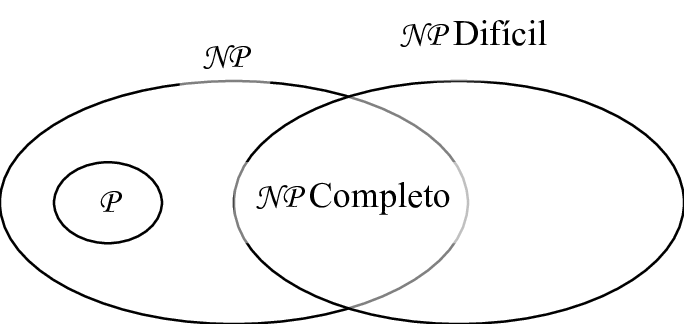
\includegraphics[width=0.5\textwidth]{img/relacaoDeConjuntos.png}
    \caption{Diagrama das classes de complexidade P, NP, NP-completo e NP-difícil.}
    \label{fig:complexidade}
\end{figure}

\subsection{Algoritmos Fundamentais}

Para avaliar o impacto das linguagens no desempenho, foram selecionados algoritmos representativos das diferentes classes polinomiais, considerando tanto sua relevância teórica quanto aplicabilidade prática.

\subsubsection{Ordenação}

O algoritmo MergeSort é representativo da classe P, com complexidade \( O(n \log n) \). Sua popularidade e ampla utilização tornam-no adequado como benchmark para linguagens compiladas e interpretadas.

\subsubsection{Problemas de Otimização e Fatoração}

O Problema da Mochila (Knapsack) foi escolhido por representar a classe NP-completo, desafiando linguagens em cenários de busca combinatória. Já a Fatoração de inteiros (Factoring), pertencente à classe NP, é relevante em aplicações como criptografia, permitindo analisar desempenho em problemas de verificação.

\subsubsection{Problemas Indecidíveis}

O Problema da Parada, embora indecidível em sua formulação geral, pode ser explorado em instâncias restritas, simulando programas com entradas controladas. Essa abordagem permite observar o comportamento das linguagens em termos de tempo de execução e uso de memória.

\subsection{Linguagens de Programação}

A linguagem de programação exerce impacto significativo na implementação de algoritmos, afetando diretamente tempo de execução, uso de memória e esforço de desenvolvimento.

\subsubsection{Critérios de Seleção}

As linguagens foram escolhidas com base em três critérios principais:

\begin{itemize}
    \item \textbf{Popularidade}: Indicadores como o TIOBE Index \citeonline{tiobe}, o GitHub Octoverse \citeonline{octoverse} e o Stack Overflow Developer Survey \citeonline{stackoverflow}.
    \item \textbf{Diversidade de paradigmas}: Inclusão de linguagens compiladas (C, C++, Rust), interpretadas (Python, JavaScript) e híbridas (Java, C\#, Go, Kotlin, TypeScript).
    \item \textbf{Aplicabilidade acadêmica e industrial}: Conforme discutido por \citeonline{sebesta2016}, essas linguagens possuem ampla adoção em contextos práticos e teóricos.
\end{itemize}

\subsubsection{Paradigmas e Modelos de Execução}

A diversidade de paradigmas cobre características essenciais para análise comparativa:

\begin{itemize}
    \item \textbf{Modelo de execução}: Compilado (execução direta) ou interpretado (via máquina virtual ou interpretador).
    \item \textbf{Tipagem}: Estática (C, Java) ou dinâmica (Python, JavaScript).
    \item \textbf{Gerenciamento de memória}: Manual (C, C++) ou automático (Java, Python).
\end{itemize}

Essas variações influenciam diretamente o desempenho e a escalabilidade, justificando a escolha do conjunto de linguagens para os experimentos.


% Materiais e Métodos
\section{Materiais e Métodos}

\subsection{Ambiente Experimental}

Os experimentos foram conduzidos em ambiente controlado, a fim de reduzir variações externas que pudessem interferir nas medições de desempenho. A configuração de hardware e software utilizada foi a seguinte:

\begin{itemize}
    \item \textbf{Processador}: Intel Core i7-1165G7 (11ª geração), 2.80 GHz, com suporte a múltiplos threads.
    \item \textbf{Memória RAM}: 16 GB DDR4 (2667 MHz).
    \item \textbf{Placa de vídeo}: Intel Iris Xe Graphics com 128 MB de memória dedicada.
    \item \textbf{Sistema operacional}: Ubuntu 22.04 LTS.
\end{itemize}

Essa infraestrutura assegurou uniformidade na execução dos algoritmos, minimizando influências externas como processos em segundo plano ou gerenciadores de energia.

\subsection{Métricas}

Foram avaliadas três métricas principais:

\begin{itemize}
    \item \textbf{Tempo de execução (Wall Clock Time)}: média de 30 execuções consecutivas, representando o tempo real decorrido, incluindo overheads do interpretador ou da máquina virtual.
    \item \textbf{Uso de memória (RSS)}: obtido por meio do utilitário \texttt{/usr/bin/time}, considerando o pico de memória residente durante a execução.
    \item \textbf{Complexidade de implementação}: mensurada por Linhas de Código Fonte (SLOC) e Complexidade Ciclomática (McCabe), como proxies de esforço de desenvolvimento e legibilidade.
\end{itemize}

A escolha dessas métricas buscou compreender não apenas o desempenho absoluto (tempo e memória), mas também o esforço associado à implementação em cada linguagem.

\subsection{Conjuntos de Dados}

Foram gerados conjuntos de dados sintéticos escaláveis, assegurando reprodutibilidade e diversidade de instâncias. Os tamanhos escolhidos refletem diferentes ordens de grandeza:

\begin{itemize}
    \item \textbf{Pequeno}: \( n = 10^3 \), representando cenários em que o overhead da linguagem pode ser mais relevante.
    \item \textbf{Médio}: \( n = 10^4 \), para avaliar comportamento intermediário e transições de eficiência.
    \item \textbf{Grande}: \( n = 10^5 \), simulando cargas intensivas e testando escalabilidade prática.
\end{itemize}

Cada instância foi gerada aleatoriamente, evitando vieses que favorecessem uma linguagem específica.

\subsection{Procedimentos Experimentais}

O procedimento experimental seguiu as seguintes etapas:

\begin{enumerate}
    \item Implementação dos algoritmos em todas as linguagens, utilizando apenas bibliotecas padrão para evitar otimizações artificiais.
    \item Compilação (para linguagens compiladas) ou execução em interpretadores com parâmetros padrão (para linguagens interpretadas).
    \item Execução repetida de cada algoritmo (30 vezes) em cada tamanho de entrada, com coleta das métricas definidas.
    \item Armazenamento e análise estatística dos resultados, considerando medidas de tendência central (média e mediana) e de variabilidade (desvio padrão).
\end{enumerate}


% 4. Resultados
\section{Resultados}

Nesta seção são apresentados os resultados obtidos a partir da execução dos experimentos descritos anteriormente. As métricas avaliadas foram: tempo médio de execução, uso de memória, consumo de CPU e complexidade de implementação (linhas de código). Para cada combinação de linguagem, tamanho do dataset e algoritmo, os testes foram repetidos 30 vezes a fim de calcular média e desvio-padrão, assegurando maior robustez estatística.

\subsection{Tempo de Execução}

A Figura~\ref{fig:tempo_execucao} apresenta a evolução do tempo de execução em função do tamanho do dataset. Observa-se que os algoritmos de classes polinomiais mantêm desempenho estável mesmo em instâncias maiores, enquanto aqueles com maior complexidade apresentaram crescimento acentuado. Os resultados confirmam a tendência teórica esperada.

\begin{figure}[H]
    \centering
    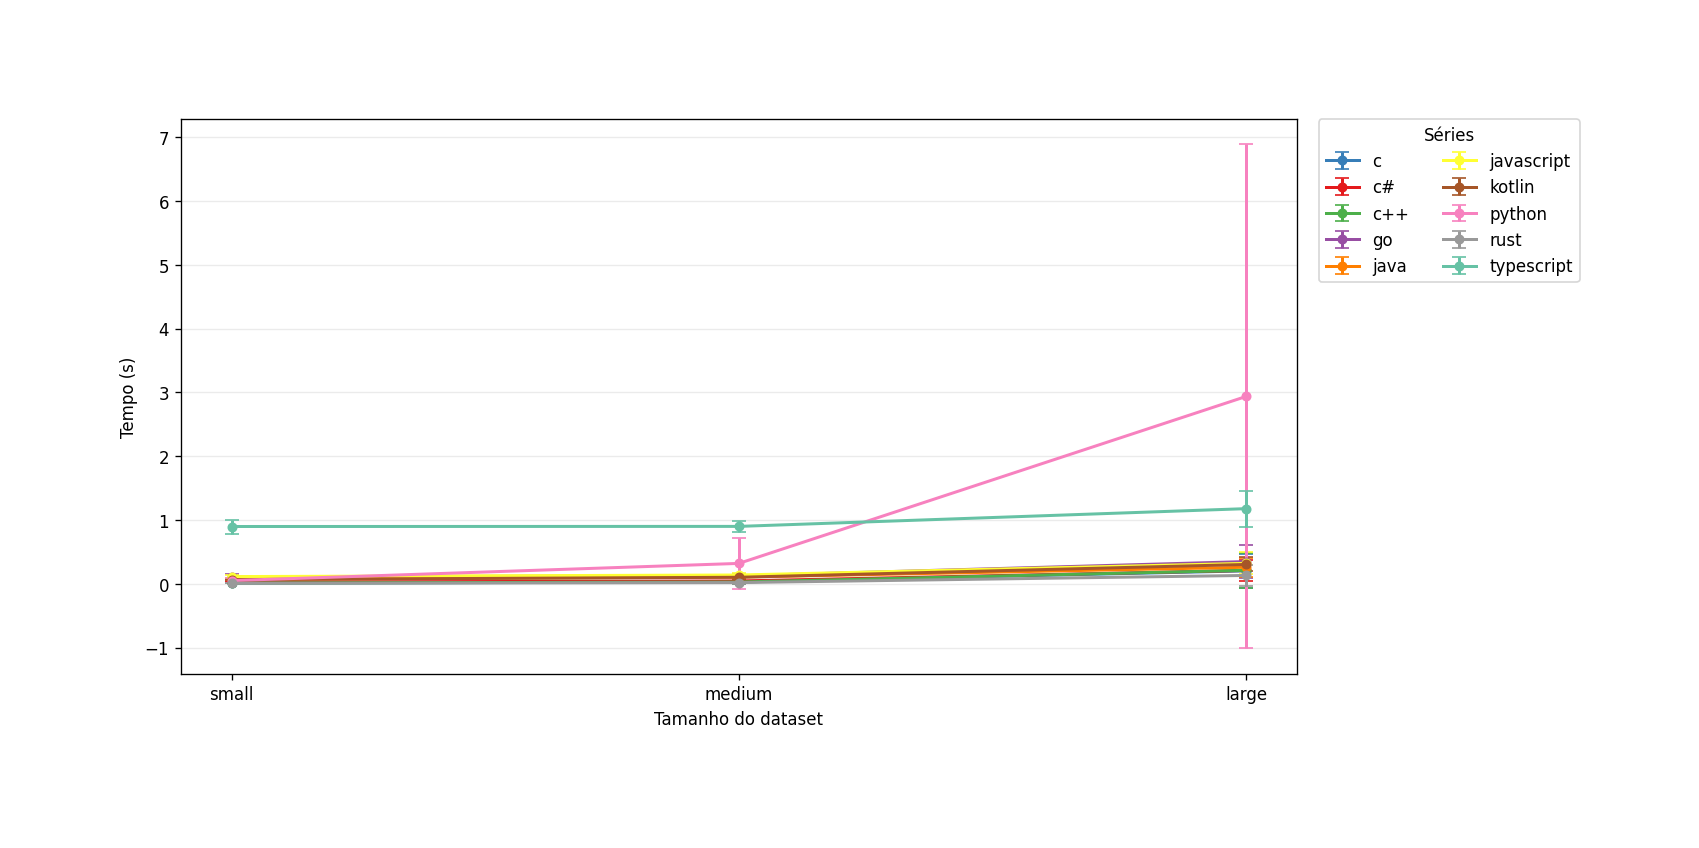
\includegraphics[width=0.8\textwidth]{img/tempo_vs_tamanho_all.png}
    \caption{Tempo médio de execução em função do tamanho do dataset (geral, sem NP-Completo). Barras indicam o desvio-padrão.}
    \label{fig:tempo_execucao}
\end{figure}

\begin{table}[H]
    \centering
    \caption{Tempo médio de execução (em segundos) e desvio-padrão por linguagem e tamanho do dataset (geral, sem NP-Completo).}
    \label{tab:tempo_execucao_geral_sem_npcomp}
    \resizebox{\textwidth}{!}{%
    \begin{tabular}{l|cc|cc|cc|cc|cc|cc|cc|cc|cc|cc|cc}
        \hline
        \textbf{Tamanho} & \multicolumn{2}{c|}{\textbf{C}} & \multicolumn{2}{c|}{\textbf{C\#}} & \multicolumn{2}{c|}{\textbf{C++}} & \multicolumn{2}{c|}{\textbf{Go}} & \multicolumn{2}{c|}{\textbf{Java}} & \multicolumn{2}{c|}{\textbf{JS}} & \multicolumn{2}{c|}{\textbf{Kotlin}} & \multicolumn{2}{c|}{\textbf{Python}} & \multicolumn{2}{c|}{\textbf{Rust}} & \multicolumn{2}{c}{\textbf{TS}} \\
        \hline
        & M & DP & M & DP & M & DP & M & DP & M & DP & M & DP & M & DP & M & DP & M & DP & M & DP \\
        \hline
        small  & 0.01 & 0.00 & 0.03 & 0.00 & 0.01 & 0.01 & 0.11 & 0.05 & 0.07 & 0.01 & 0.11 & 0.02 & 0.07 & 0.01 & 0.05 & 0.04 & 0.01 & 0.00 & 0.90 & 0.11 \\
        medium & 0.03 & 0.03 & 0.04 & 0.02 & 0.03 & 0.03 & 0.12 & 0.03 & 0.10 & 0.02 & 0.14 & 0.03 & 0.10 & 0.01 & 0.32 & 0.40 & 0.02 & 0.02 & 0.90 & 0.09 \\
        large  & 0.20 & 0.27 & 0.21 & 0.17 & 0.21 & 0.28 & 0.35 & 0.26 & 0.26 & 0.26 & 0.32 & 0.17 & 0.30 & 0.11 & 2.94 & 3.95 & 0.13 & 0.16 & 1.18 & 0.28 \\
        \hline
    \end{tabular}%
    }
\end{table}

\textbf{Conclusão parcial:} Linguagens compiladas de baixo nível (C, C++, Rust) apresentaram tempos de execução consistentes e reduzidos em todos os tamanhos de dataset, evidenciando maior eficiência. Em contraste, Python e TypeScript exibiram desempenho inferior, especialmente em instâncias grandes, refletindo limitações inerentes a modelos de execução interpretados.

\subsection{Uso de CPU}

A Figura~\ref{fig:cpu} mostra o consumo máximo de CPU normalizada durante as execuções. O aumento é mais pronunciado nos datasets maiores, indicando maior esforço computacional para manter os cálculos.

\begin{figure}[H]
    \centering
    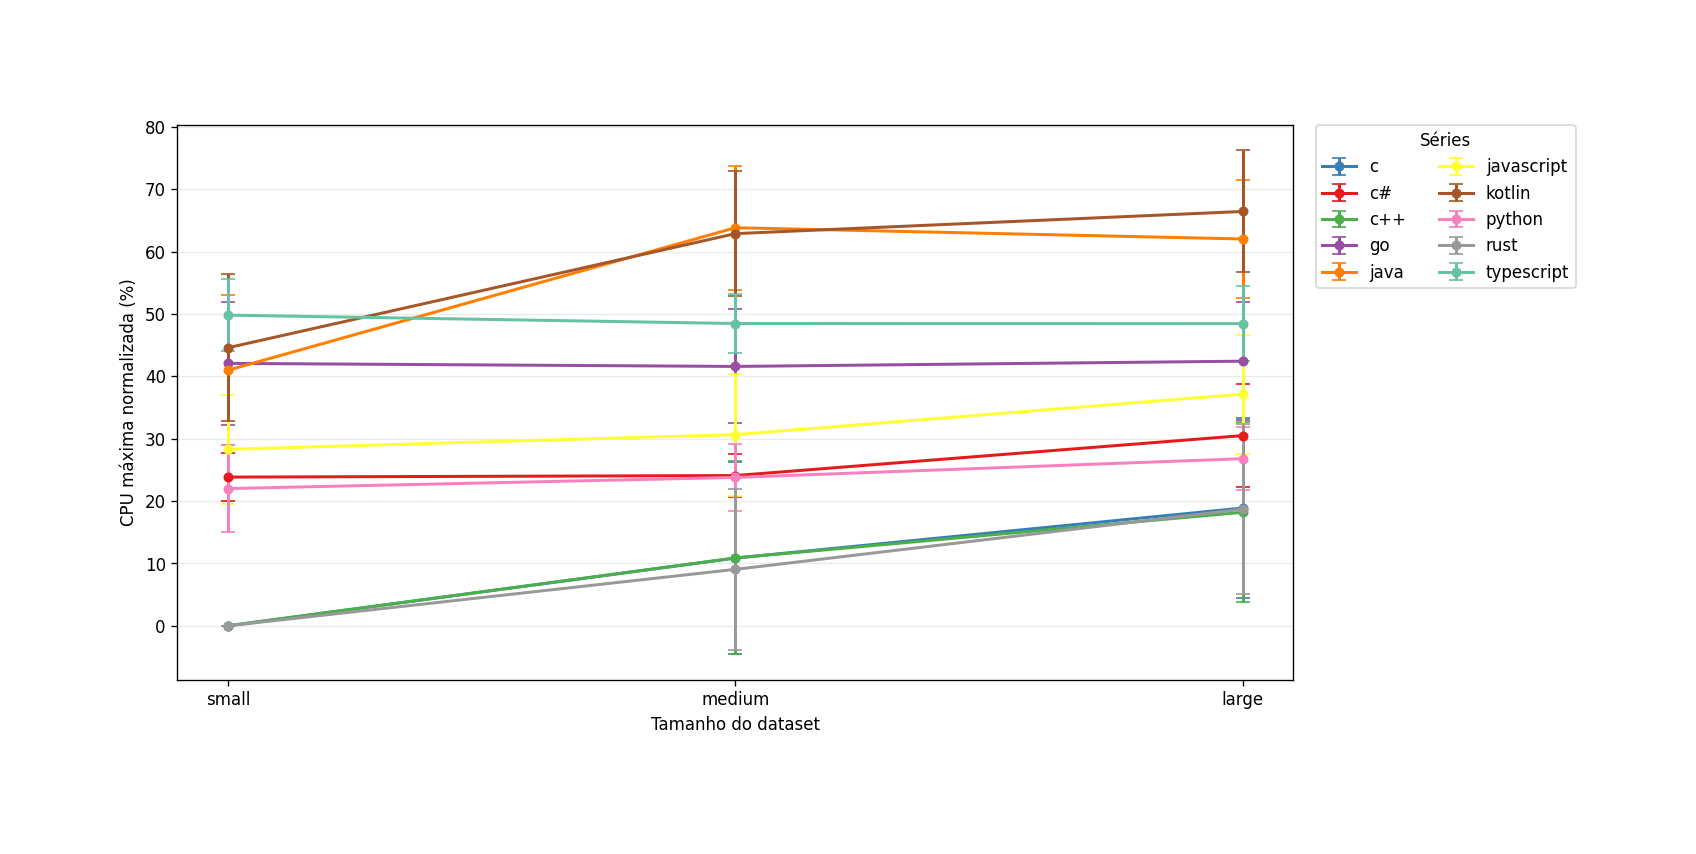
\includegraphics[width=0.8\textwidth]{img/cpu_vs_tamanho_all.png}
    \caption{Consumo máximo de CPU normalizada para cada tamanho de dataset.}
    \label{fig:cpu}
\end{figure}

\begin{table}[H]
    \centering
    \caption{Consumo máximo de CPU normalizada (\%) por linguagem e tamanho de dataset.}
    \label{tab:cpu}
    \resizebox{\textwidth}{!}{%
    \begin{tabular}{l|cc|cc|cc|cc|cc|cc|cc|cc|cc|cc|cc}
        \hline
        \textbf{Tamanho} & \multicolumn{2}{c|}{\textbf{C}} & \multicolumn{2}{c|}{\textbf{C\#}} & \multicolumn{2}{c|}{\textbf{C++}} & \multicolumn{2}{c|}{\textbf{Go}} & \multicolumn{2}{c|}{\textbf{Java}} & \multicolumn{2}{c|}{\textbf{JS}} & \multicolumn{2}{c|}{\textbf{Kotlin}} & \multicolumn{2}{c|}{\textbf{Py}} & \multicolumn{2}{c|}{\textbf{Rust}} & \multicolumn{2}{c}{\textbf{TS}} \\
        & M & DP & M & DP & M & DP & M & DP & M & DP & M & DP & M & DP & M & DP & M & DP & M & DP \\
        \hline
        small  & 0.00 & 0.00 & 23.84 & 3.86 & 0.00 & 0.00 & 42.08 & 9.85 & 40.99 & 12.08 & 28.30 & 8.78 & 44.59 & 11.82 & 22.00 & 7.01 & 0.00 & 0.00 & 49.82 & 5.72 \\
        medium & 10.86 & 15.46 & 24.09 & 3.43 & 10.88 & 15.48 & 41.59 & 9.14 & 63.83 & 9.91 & 30.66 & 9.79 & 62.89 & 10.08 & 23.79 & 5.35 & 9.05 & 12.91 & 48.47 & 4.76 \\
        large  & 18.88 & 14.40 & 30.50 & 8.21 & 18.21 & 14.42 & 42.43 & 9.46 & 62.03 & 9.42 & 37.15 & 9.55 & 66.44 & 9.78 & 26.79 & 5.04 & 18.70 & 13.65 & 48.45 & 6.07 \\
        \hline
    \end{tabular}%
    }
\end{table}

\textbf{Conclusão parcial:} Go, Kotlin e Java apresentaram maior consumo de CPU em instâncias grandes, reflexo do overhead de suas máquinas virtuais. Já C e C++ destacaram-se pelo uso mais eficiente de processamento. Python exibiu elevada variação, indicando menor previsibilidade no uso de recursos.

\subsection{Uso de Memória}

O consumo de memória é apresentado na Figura~\ref{fig:memoria}. Verifica-se aumento gradual com o crescimento do dataset, sendo mais acentuado em linguagens com ambientes de execução mais pesados (Java, Kotlin, TypeScript).

\begin{figure}[H]
    \centering
    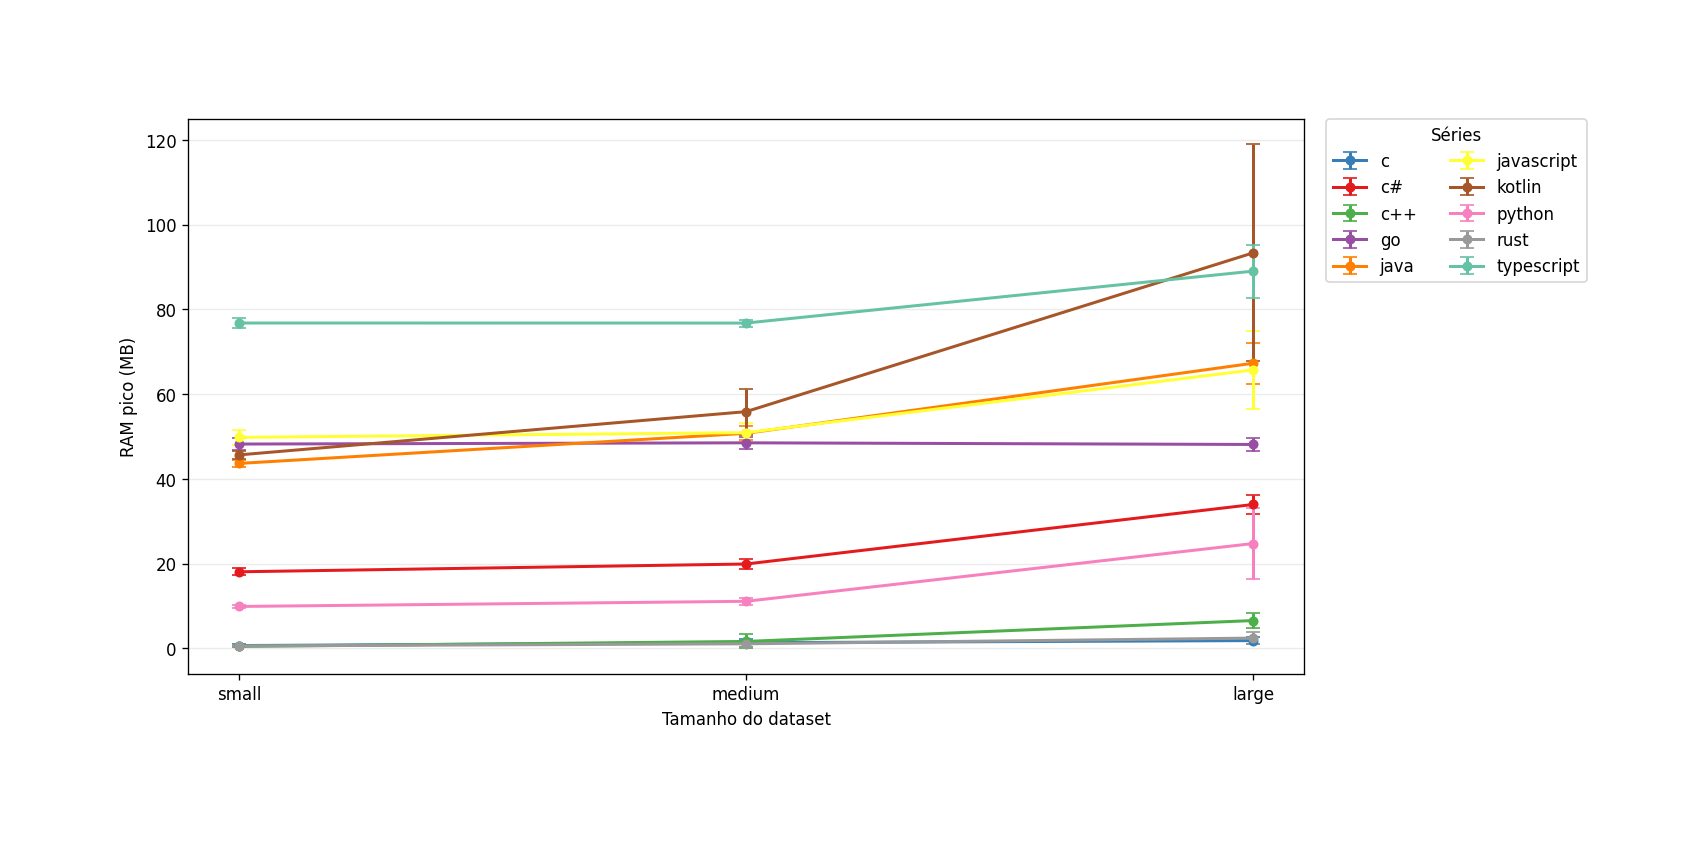
\includegraphics[width=0.8\textwidth]{img/ram_vs_tamanho_all.png}
    \caption{Uso máximo de memória em função do tamanho do dataset.}
    \label{fig:memoria}
\end{figure}

\begin{table}[H]
    \centering
    \caption{Uso máximo de memória (MB) e desvio padrão (DP).}
    \label{tab:memoria}
    \resizebox{\textwidth}{!}{%
        \begin{tabular}{c|cc|cc|cc|cc|cc|cc|cc|cc|cc|cc}
            \hline
            \textbf{Tamanho}
            & \multicolumn{2}{c|}{\textbf{C}}
            & \multicolumn{2}{c|}{\textbf{C\#}}
            & \multicolumn{2}{c|}{\textbf{C++}}
            & \multicolumn{2}{c|}{\textbf{Go}}
            & \multicolumn{2}{c|}{\textbf{Java}}
            & \multicolumn{2}{c|}{\textbf{JS}}
            & \multicolumn{2}{c|}{\textbf{Kotlin}}
            & \multicolumn{2}{c|}{\textbf{Py}}
            & \multicolumn{2}{c|}{\textbf{Rust}}
            & \multicolumn{2}{c}{\textbf{TS}} \\
            \cline{2-21}
            & M & DP & M & DP & M & DP & M & DP & M & DP & M & DP & M & DP & M & DP & M & DP & M & DP \\
            \hline
            small  & 0.68 & 0.29 & 18.08 & 0.81 & 0.48 & 0.06 & 48.23 & 1.51 & 43.65 & 0.80 & 49.80 & 1.70 & 45.66 & 0.87 & 9.90 & 0.41 & 0.58 & 0.30 & 76.78 & 1.29 \\
            medium & 1.35 & 0.94 & 19.92 & 1.25 & 1.65 & 1.66 & 48.52 & 1.46 & 50.76 & 1.62 & 50.92 & 2.22 & 55.87 & 5.43 & 11.12 & 0.79 & 1.09 & 0.75 & 76.78 & 0.82 \\
            large  & 1.85 & 0.86 & 33.97 & 2.18 & 6.58 & 1.86 & 48.13 & 1.49 & 67.30 & 4.80 & 65.73 & 9.21 & 93.35 & 25.56 & 24.76 & 8.39 & 2.44 & 1.46 & 89.03 & 6.27 \\
            \hline
        \end{tabular}%
    }
\end{table}

\textbf{Conclusão parcial:} C e C++ demonstraram consumo mínimo de memória, reforçando sua eficiência em cenários críticos. Em contraste, Java, Kotlin e TypeScript apresentaram demandas mais elevadas, refletindo os custos adicionais de suas máquinas virtuais.

\subsection{Qualidade da Solução da Heurística}

Nos conjuntos menores (\(n = 10^3\) e \(n = 10^4\)), foi possível comparar diretamente o desempenho do algoritmo heurístico em relação ao exato. Observa-se que a heurística reduziu drasticamente o tempo de execução, com perda mínima de qualidade. Para o conjunto grande, apenas o heurístico pôde ser avaliado.

\begin{figure}[H]
    \centering
    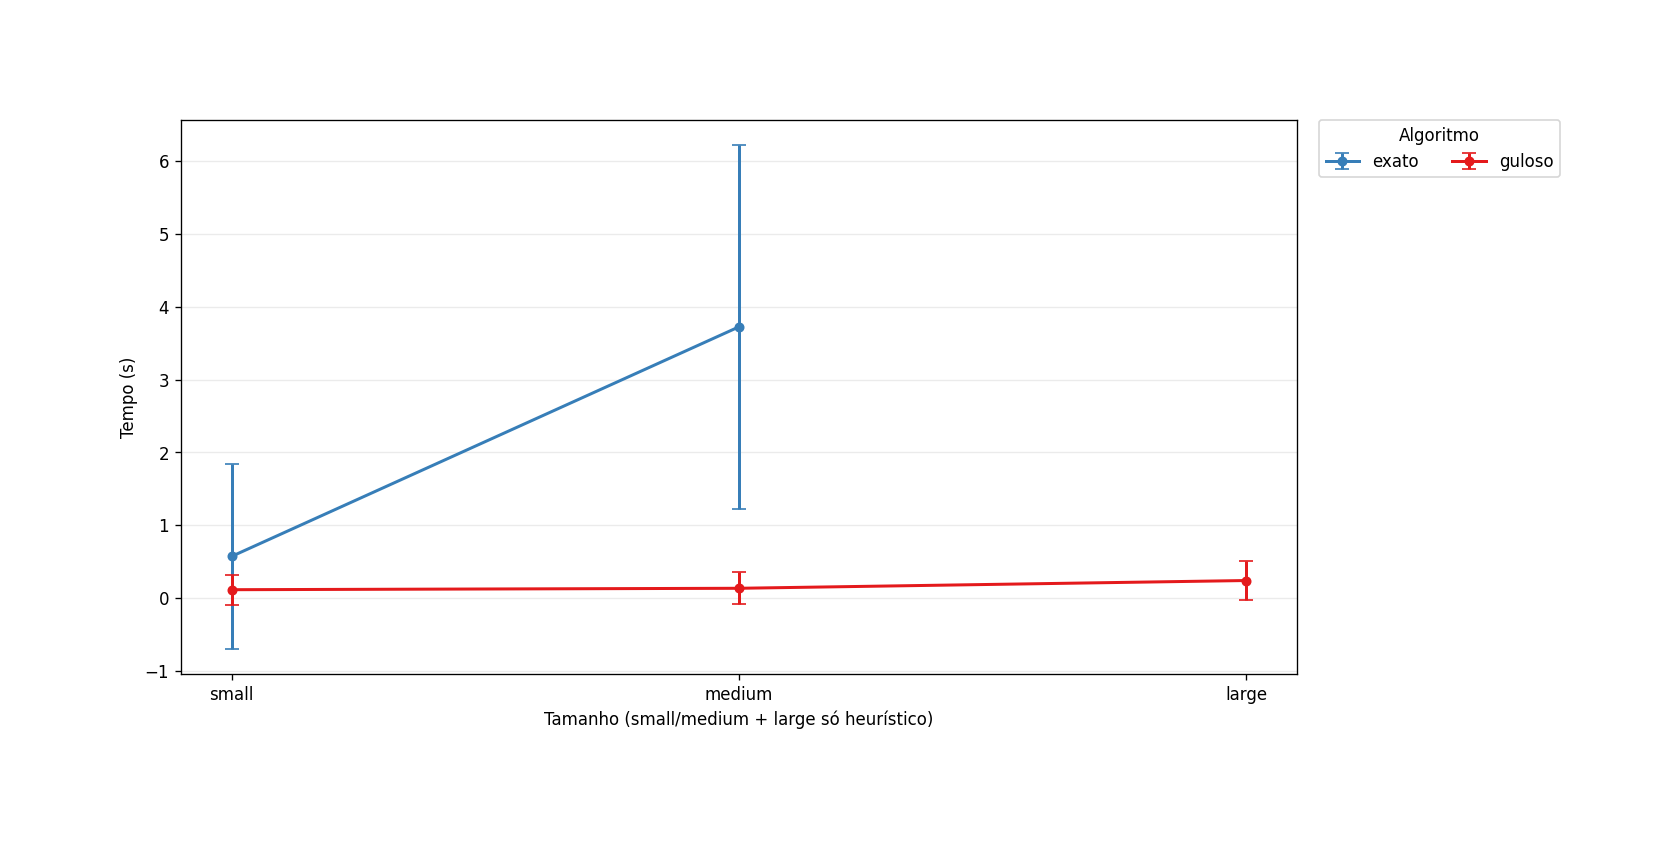
\includegraphics[width=0.8\textwidth]{img/qualidade_heuristica.png}
    \caption{Comparação de tempo de execução entre solução exata e heurística (NP-Completo).}
    \label{fig:qualidade}
\end{figure}

\begin{table}[H]
    \centering
    \caption{Comparação de tempo de execução entre solução exata e heurística (NP-Completo).}
    \label{tab:qualidade_np}
    \resizebox{0.8\textwidth}{!}{%
    \begin{tabular}{c|cc|cc}
        \hline
        \textbf{Tamanho} & \multicolumn{2}{c|}{\textbf{Exato}} & \multicolumn{2}{c}{\textbf{Heurístico (Guloso)}} \\
        \cline{2-5}
         & M (s) & DP (s) & M (s) & DP (s) \\
        \hline
        small  & 0.57 & 1.27 & 0.11 & 0.21 \\
        medium & 3.72 & 2.50 & 0.13 & 0.22 \\
        large  & -- & -- & 0.24 & 0.26 \\
        \hline
    \end{tabular}%
    }
\end{table}

\textbf{Conclusão parcial:} A heurística apresentou ganhos expressivos em tempo de execução, sobretudo nos datasets médios, com perdas mínimas em relação à solução ótima. Nas instâncias grandes, o algoritmo exato tornou-se inviável, enquanto a heurística manteve tempos baixos e escalabilidade.

\subsection{Linhas de Código}

A Figura~\ref{fig:sloc} e a Tabela~\ref{tab:sloc} apresentam a quantidade média de linhas de código (SLOC) necessárias para implementar cada algoritmo em cada linguagem. Essa métrica reflete a complexidade de implementação e serve de base para discutir o trade-off entre facilidade de desenvolvimento e desempenho.

\begin{figure}[H]
    \centering
    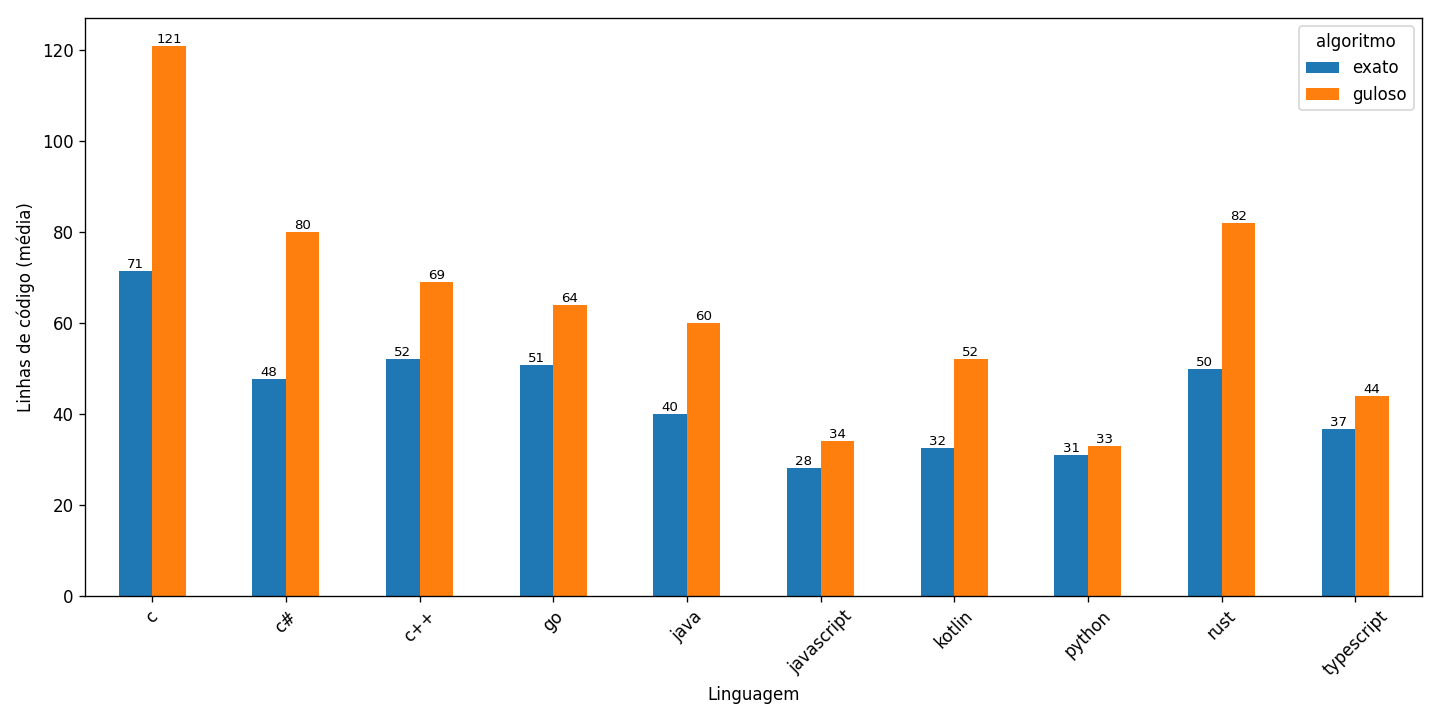
\includegraphics[width=0.8\textwidth]{img/linhas_codigo_linguagem_algoritmo.png}
    \caption{Linhas de código (SLOC) médias por linguagem e algoritmo.}
    \label{fig:sloc}
\end{figure}

\begin{table}[H]
    \centering
    \caption{Linhas de código (SLOC) médias por linguagem e algoritmo.}
    \label{tab:sloc}
    \resizebox{0.7\textwidth}{!}{%
        \begin{tabular}{c|c|c}
            \hline
            \textbf{Linguagem} & \textbf{Algoritmo Exato} & \textbf{Algoritmo Heurístico} \\
            \hline
            C          & 71 & 121 \\
            C\#        & 48 & 80 \\
            C++        & 52 & 69 \\
            Go         & 51 & 64 \\
            Java       & 40 & 60 \\
            JavaScript & 28 & 34 \\
            Kotlin     & 32 & 52 \\
            Python     & 31 & 33 \\
            Rust       & 50 & 82 \\
            TypeScript & 37 & 44 \\
            \hline
        \end{tabular}%
    }
\end{table}

\textbf{Conclusão parcial:} Python e JavaScript demandaram menos linhas de código, revelando maior expressividade e simplicidade na implementação. Em contrapartida, C e Rust exigiram códigos mais extensos, refletindo maior controle sobre aspectos de baixo nível.

\vspace{0.3cm}
\subsection{Síntese Geral dos Resultados}

De modo geral, os resultados confirmam que linguagens compiladas (C, C++, Rust) são mais adequadas para cenários que exigem alta eficiência em tempo e memória, enquanto linguagens interpretadas (Python, JavaScript, TypeScript) oferecem maior produtividade e expressividade às custas de menor desempenho. Java, Go e Kotlin apresentaram comportamento intermediário, beneficiados por suas máquinas virtuais, mas com custos adicionais de CPU e memória. 

A heurística demonstrou-se uma solução viável para problemas NP-Completo, conciliando rapidez e qualidade aceitável das soluções. Assim, os achados reforçam que a escolha da linguagem deve considerar não apenas desempenho, mas também o equilíbrio entre recursos computacionais disponíveis, tempo de desenvolvimento e requisitos práticos da aplicação.


% 5. Conclusão
\section{Conclusão}
Este trabalho apresentou uma análise comparativa de algoritmos implementados em diferentes linguagens de programação, com foco em métricas de desempenho (tempo de execução, uso de CPU e memória) e complexidade de implementação (linhas de código). O objetivo central foi investigar o impacto da linguagem de programação na eficiência computacional, considerando cenários controlados e instâncias de diferentes tamanhos.

Os resultados evidenciaram que linguagens compiladas de baixo nível, como C, C++ e Rust, mantiveram desempenho superior em termos de tempo e memória, confirmando sua adequação a aplicações que demandam alta eficiência. Em contrapartida, linguagens interpretadas como Python, JavaScript e TypeScript, embora apresentem menor desempenho em grandes volumes de dados, destacaram-se pela simplicidade de implementação e expressividade. Linguagens intermediárias, como Java, Kotlin e Go, mostraram um equilíbrio entre desempenho e produtividade, mas com custo adicional em consumo de CPU e memória devido ao uso de máquinas virtuais.

De forma aplicada, os resultados sugerem que a escolha da linguagem deve considerar o contexto do problema. Para cenários que exigem alto desempenho e baixo consumo de recursos, como sistemas embarcados, computação científica e aplicações em tempo real, linguagens compiladas de baixo nível (C, C++ e Rust) são mais indicadas. Em ambientes corporativos ou acadêmicos, onde a produtividade, a clareza do código e a facilidade de manutenção têm maior peso, linguagens como Python e JavaScript oferecem vantagens, ainda que com menor eficiência em escala. Já linguagens intermediárias, como Java, Kotlin e Go, mostram-se adequadas para sistemas distribuídos e aplicações de larga escala, em que o equilíbrio entre desempenho e portabilidade é determinante.

A análise da heurística aplicada ao problema NP-Completo demonstrou que abordagens aproximadas oferecem soluções próximas ao ótimo em frações do tempo exigido pelo algoritmo exato, viabilizando aplicações práticas em cenários de maior escala. Esse achado reforça o trade-off entre precisão e eficiência computacional, fundamental em problemas de alta complexidade.

Como limitações, destaca-se a utilização de um único ambiente experimental, o que restringe a generalização dos resultados para diferentes arquiteturas de hardware e sistemas operacionais. Ademais, foram considerados apenas algoritmos representativos das classes P, NP, NP-Completo e NP-difícil, não abrangendo a totalidade do espectro de problemas computacionais.

Como perspectivas futuras, propõe-se ampliar os experimentos para incluir diferentes configurações de hardware, explorar métricas adicionais como consumo energético e escalabilidade em ambientes distribuídos, além de avaliar outras linguagens emergentes e paradigmas de programação. Tais investigações podem aprofundar a compreensão dos impactos da linguagem de programação no desempenho e orientar decisões ainda mais embasadas em contextos acadêmicos e industriais.


% REFERÊNCIAS
\bibliographystyle{abntex2-alf}
\bibliography{Bibliografia}

\end{document}
